\documentclass[11pt,a4paper,twocolumn]{article}

% === Packages ===
\usepackage[utf8]{inputenc}
\usepackage[T1]{fontenc}
\usepackage{microtype}
\usepackage{amsmath,amssymb}
\usepackage{booktabs}
\usepackage{graphicx}
\usepackage{xcolor}
\usepackage{listings}
\usepackage{needspace}
\usepackage{url}
\usepackage[numbers]{natbib}
\usepackage[hidelinks]{hyperref}
\usepackage{tikz}
\usepackage{pgfplots}
\pgfplotsset{compat=1.18}
\usetikzlibrary{positioning, arrows.meta, fit, backgrounds, calc, shapes.geometric}

\graphicspath{{figures/}}

% Listings style for code excerpts
\lstset{
  basicstyle=\ttfamily\small,
  breaklines=true,
  frame=single,
  columns=fullflexible,
  keepspaces=true,
  showstringspaces=false
}

% === Front matter ===
\title{Entmoot: Social Group Communication \\
       for Autonomous Agents \\
       over Pilot Protocol}

\author{%
  Jerry Fanelli\\
  \texttt{jerry.fanelli@gmail.com}%
}

\date{\today}

\begin{document}
\maketitle

\begin{abstract}
Entmoot is a durable group-communication substrate for autonomous agents that
already have pairwise identity and trust. Its main empirical result is
convergence after a real residential-edge partition: in a 120-hour live run
across a VPS, two container runtimes, and a Raspberry Pi, all four nodes
finished with healthy diagnostics and the same controlled group state
(4 members, 78 controlled-topic messages). The recovery window for the
longest Phobos outage is bounded only at snapshot granularity: the last
unhealthy checkpoint was 20260606T052015Z and the first subsequent checkpoint
showing the full controlled state was 20260606T054137Z, a 21.37-minute bound,
not a delivery-latency measurement. Entmoot represents a group, or
\emph{moot}, as signed membership state plus signed messages propagated by
gossip and repaired by anti-entropy reconciliation. The reference Go
implementation runs over Pilot Protocol as the deployed pairwise-trust
overlay, but the design target is more general: signed group conversation
above trust-gated agent transports. It provides private and public moots,
targeted and open invites, founder-managed policies, an Entmoot Service
Provider (ESP) surface for web and mobile clients, lexical search with
message-context jumps, and Agent Skills plus Codex/Claude plugin packaging for
agent-facing use.
\end{abstract}

% === 1. Introduction ===
\section{Introduction}
\label{sec:introduction}

Autonomous agents increasingly need communication that is neither a
single-tool RPC nor a centralized orchestrator. Recent agent-protocol work
standardizes tool access, task delegation, discovery, direct messaging, and
cross-domain interoperation~\citep{ehtesham2025interopSurvey,anpMessaging2026},
while recent gossip-for-agents papers argue that decentralized dissemination
is a missing substrate for adaptive multi-agent coordination
~\citep{habiba2025gossipVision,khan2025gossipSubstrate}. Entmoot takes the
next systems step: it implements a deployed signed group conversation layer
over a pairwise-trust agent overlay and evaluates whether that layer converges
after real operational disruption.

Pilot Protocol is the deployed overlay used in this paper, not the premise of
the design. In an empirical study of the Pilot network, agents registered,
handshook, exchanged trust, and formed a topology with heavy-tailed degree
distribution, 47$\times$ higher clustering than random, and a giant component
spanning two-thirds of the population~\citep{calin2026emergent}. That result
is useful because Pilot offers the lower-layer primitives that many agent
overlays need: identity, discovery, trust, NAT traversal, and encrypted
1-to-1 streams. What persists across more than two peers is left to
applications.

The missing primitive is a durable group conversation. A pairwise overlay can
connect agents, but it does not by itself answer group questions: who belongs
to a room, who may invite new members, which messages were sent on a topic,
how intermittent clients catch up, how a public room is discovered, or how an
agent searches shared history after the fact. An agent that wants to address a
dozen peers can maintain individual relationships with all of them, or it can
delegate group state to a centralized service. The first approach scales
poorly as a social practice; the second undermines the decentralized trust
model that made the Pilot graph interesting in the first place.

Entmoot adds that group layer without replacing the pairwise overlay. A group, or
\emph{moot}, consists of signed roster state, signed messages, optional
invites, policy metadata, and a gossip/reconciliation protocol that moves data
over ordinary reliable streams. Members can participate directly, while an
Entmoot Service Provider (ESP) can project the same group state to web and
mobile clients without becoming the source of group truth. Public moot
descriptors make opt-in communities discoverable, but public visibility is
separate from message history, live replies, and membership consent.

The current implementation is social-first. It supports private and public
moots, default and founder-customized policies, searchable history,
message-context jumps from search results back into chat, member profiles and
display names, owner-controlled live-agent replies, and an Agent
Skills-compatible packaging surface for Codex, Claude, and OpenClaw-style
agents. Fleet and task coordination exist only as opt-in extensions and are
disabled by default. This framing matters: Entmoot is not primarily a job
orchestrator. It is a shared social memory and conversation layer for agents.

Our contributions are as follows.

\begin{enumerate}
    \item A signed moot model for group communication over pairwise-trust
    agent overlays, instantiated over Pilot, including member identities,
    rosters, targeted invites, open invites, signed messages, topic routing,
    and founder/admin authority.
    \item A dissemination and repair design that combines Pilot streams,
    gossip fanout, replay protection, rate limiting, Merkle roots, and
    anti-entropy reconciliation to make group history durable across
    intermittently connected agents.
    \item An ESP architecture that exposes group state to web and mobile
    clients while preserving the distinction between signed group state and
    ESP-local convenience state such as device auth, cursors, profiles, and
    display names.
    \item Public discovery and governance mechanisms: public moot descriptors,
    ESP directory indexing, consent-first joins, default policies, and
    founder-managed policy updates.
    \item Agent-facing packaging through an Agent Skills document and
    Codex/Claude plugin generation, so autonomous coding agents can discover,
    install, diagnose, and use Entmoot as a chat substrate.
    \item A five-day empirical evaluation that measures multi-runtime
    monitoring, controlled-topic delivery, transcript export, and
    convergence-after-partition behavior across heterogeneous agent runtimes.
    \item A lab-scale in-memory benchmark harness, following the GossipSub
    evaluation template's focus on delivery distribution, duplicate delivery,
    loss, repair bandwidth, and join catch-up~\citep{vyzovitis2020gossipsub}.
\end{enumerate}

The rest of the paper is organized as follows. Section~\ref{sec:background}
positions Entmoot against Pilot, pub/sub, social, gossip, and log-repair
systems. Section~\ref{sec:model} defines the system model and trust
boundaries. Sections~\ref{sec:design} and~\ref{sec:implementation} describe
the protocol and implementation. Sections~\ref{sec:evaluation}
and~\ref{sec:results} separate the evaluation method from the results.
Sections~\ref{sec:discussion},~\ref{sec:limitations},
and~\ref{sec:artifacts} discuss the implications, limits, and artifact
record before the future-work and conclusion sections.

% === 2. Background and Related Work ===
\section{Background and Related Work}
\label{sec:background}

\subsection{Pilot Protocol}

Pilot is an overlay network stack for autonomous agents~\citep{pilotprotocol}.
Each participating node generates an Ed25519 identity~\citep{bernstein2012ed25519,rfc8032}
at registration and receives a 48-bit virtual address of the form
\texttt{N:NNNN.HHHH.LLLL}: a 16-bit network ID and a 32-bit node ID within
that network. Network~0 is the global backbone; all agents are members of
it by default. Pilot reserves additional network IDs for purpose-specific
subgraphs; the \emph{Pilot Networks} feature that populates them is in
early-access release as of this writing. A Pilot Network is a
group-scoped \emph{connectivity} primitive: membership grants pairwise
authorization (``address resolution, connection acceptance, and
datagram delivery''~\citep{pilotprotocol}) between members without
requiring $O(N^2)$ bilateral handshakes. It is not a messaging layer:
Pilot Networks do not define a broadcast primitive, an ordered log,
retention, or completeness proofs --- datagrams between network
members are still point-to-point and stateless. Entmoot and Pilot
Networks are therefore complementary rather than overlapping: Pilot
Networks can eventually replace Entmoot's signed roster as the
membership source of truth (\S\ref{sec:future}), while Entmoot
contributes the broadcast semantics --- fanout, Merkle-verified
completeness, and anti-entropy reconciliation --- that a Network
membership primitive alone does not provide.

Communication is trust-gated. Two nodes must complete a cryptographic
handshake (port~444) mediated by the registry before they can exchange
traffic on any other port~\citep{calin2026emergent}. Once trust is
established, nodes may open a reliable byte stream to each other on any
port. Under the hood, Pilot runs a TCP-equivalent reliable-delivery
protocol with X25519 key exchange~\citep{rfc7748} and AES-256-GCM
authenticated encryption~\citep{nist80038d} per tunnel, the same
primitives that underlie WireGuard~\citep{donenfeld2017wireguard}. The bytes
that carry a tunnel move through a pluggable transport layer: UDP is the
default byte-mover and is what
UDP-capable peers use end-to-end, but the fork we build against also
ships a TCP transport that a public-IP daemon can expose alongside UDP
so peers on UDP-hostile networks (restrictive corporate firewalls,
carrier-grade NAT, UDP-blocking ISPs) can still establish tunnels. The
transport choice is invisible above the tunnel layer: the same wire
frames travel over whichever transport the dialing peer's direct-UDP
retries settle on. The registry does not see tunnel payloads; it only
mediates address allocation, hostname resolution, the handshake relay,
and, when present, the per-peer list of transport endpoints.

Crucially, the registry hides the network endpoint of any node not
flagged as ``public.'' A private node's address can only be resolved to
a reachable endpoint by another node with an existing trust edge. A new
participant cannot therefore bootstrap into an otherwise-private group
without either an out-of-band introduction or at least one public
introducer.

We build against the \texttt{jerryfane/pilotprotocol}
fork~\citep{pilotprotocol}, which layers a pluggable transport
abstraction and a cluster of reliability fixes on top of upstream
v1.7.2. The fork now includes NAT-drift-resilient endpoint refresh
(a STUN-style guard against carrier NAT remapping~\citep{rfc8489}),
TURN client routing for peers behind symmetric NAT~\citep{rfc8656},
strict \texttt{-outbound-turn-only} privacy mode, a small rendezvous
service for TURN-endpoint discovery, periodic peer re-lookup, TURN
permission refresh/self-heal, explicit virtual-stream lifecycle
tracing, and a self-dial guard at the transport layer
(\S\ref{sec:security}). Entmoot treats these as lower-layer
capabilities: rendezvous discovers endpoints, Pilot chooses and
executes routes, and Entmoot consumes only reliable Pilot streams and
the daemon IPC surface. The companion evolution
paper~\citep{entmootevolution} records the incident-level narrative
of how these were surfaced in live deployment and shaped the fanout,
multiplexing, anti-entropy, and recovery policies described
in~\S\ref{sec:design}.

\subsection{Autonomous agent networks}

Classical multi-agent systems literature~\citep{wooldridge2009,shohamleyton2008,dorri2018}
models agents, strategies, and coordination protocols, but it usually assumes
that the interaction topology and communication substrate are already given.
\citet{calin2026emergent} instead observes a deployed agent population on
Pilot, where the topology itself emerges from trust and discovery decisions:
agents form heavy-tailed degree distributions consistent with preferential
attachment~\citep{barabasi1999}, clustering coefficient $\sim$47$\times$
above random, and small-world
properties~\citep{watts1998small}. Functional clusters such as
data/analytics, wellness, career, and engineering emerge without a global
planner. That study also identifies a limit: all observed agents remain on
Pilot network~0, so community structure beyond pairwise trust is not yet a
first-class protocol object. Entmoot instantiates that missing group substrate.

Agent communication languages have a longer lineage. KQML and FIPA-ACL define
performative-based agent messages and message structure
~\citep{finin1994kqml,fipa2002acl}; the current interoperability wave
standardizes tool and task surfaces such as MCP, ACP, A2A, and ANP
~\citep{ehtesham2025interopSurvey}. ACP has since joined A2A under the Linux
Foundation~\citep{lfai2025acpA2A}. These protocols are complementary to
Entmoot: they help agents call tools, delegate tasks, discover capabilities,
or exchange direct messages, but they do not by themselves provide a durable
group conversation with signed membership, topic history, and repair after
partitions.

Recent agent-society work studies what happens once many language-model
agents share environments or persistent memories. Generative Agents showed
that memory, reflection, and planning can produce believable social behavior
in a small simulated town~\citep{park2023generativeAgents}; AgentSociety
scales this style of simulation to more than 10,000 LLM-driven agents and
millions of interactions~\citep{piao2025agentsociety}. Entmoot is lower in
the stack. It does not model behavior; it supplies a signed substrate on
which agents and humans can observe, search, and recover shared conversation
state.

\subsection{Nearest agent-network neighbors}

The closest recent papers make the same substrate question explicit.
\citet{habiba2025gossipVision} argue that gossip is a natural coordination
mechanism for agentic multi-agent systems and identify cryptographic
signatures and trust as needed extensions. \citet{khan2025gossipSubstrate}
propose a gossip-enhanced substrate for decentralized agentic AI. Entmoot
differs by shipping the signed, trust-gated group layer those papers motivate:
founder-signed rosters, author-signed messages, policy state, gossip,
anti-entropy repair, and a live heterogeneous deployment. ANP specifies an
end-to-end instant-messaging profile~\citep{anpMessaging2026}, Coral Protocol
frames open infrastructure for an Internet of Agents~\citep{georgio2025coral},
and AIOS AgentSites proposes Internet-scale agent-hosting sites
~\citep{zhang2025agentsites}. Entmoot's narrower contribution is not another
agent hosting or interop framework; it is durable group conversation over a
pairwise-trust overlay.

\subsection{Group messaging, pub/sub, and social protocols}

Existing messaging systems supply useful contrasts. MQTT defines hierarchical
topics and wildcard filters~\citep{mqtt5}; NATS uses subject-based
publish/subscribe for one-to-many distribution~\citep{natsPubSub}; Matrix
specifies federated rooms, event graphs, and client/server access
patterns~\citep{matrixSpec}; and ActivityPub standardizes federated social
inbox/outbox delivery~\citep{activitypub}. Entmoot borrows the idea that
messages need addressable topics and client-facing projections, but differs in
where authority sits. It is not a brokered pub/sub system like MQTT or NATS,
and its ESP layer is not the canonical home server of a Matrix-style room.
Signed rosters, signed messages, public descriptors, and reconciliation remain
verifiable outside the service that presents them to a web or mobile client.
Compared with ActivityPub, Entmoot is less a federated object-delivery protocol
than a trust-gated group log for autonomous agents already connected by Pilot.
Nostr is an additional deployed contrast: NIP-77 shows that set
reconciliation is already relevant in decentralized social systems
~\citep{negentropyNIP77}. Bluesky and the AT Protocol show a different
deployed tradeoff: usable decentralized social media built around personal
data servers and repository synchronization~\citep{kleppmann2024bluesky}.
Entmoot uses social-network lessons, but its unit of authority is a signed
agent group rather than a human account repository or relay-indexed event set.

\subsection{Gossip, logs, and reconciliation}

Entmoot's dissemination layer follows the long line of epidemic
replication~\citep{demers1987epidemic} and gossip broadcast. Plumtree supplies
the eager/lazy tree-repair pattern~\citep{leitao2007plumtree}; libp2p
GossipSub adapts mesh gossip and peer scoring for large public
networks~\citep{gossipsubSpec,vyzovitis2020gossipsub}. Entmoot uses the same
general separation between fast-path push and repair, but at smaller
trust-scoped group boundaries and over Pilot streams rather than libp2p
connections. Secure Scuttlebutt is a closer log-structured peer: it uses
per-identity signed append-only logs and gossip repair~\citep{tarr2019ssb}.
Entmoot differs by making the group, not only the author, a signed object with
membership, invite, policy, and public-discovery state.

Merkle logs and content addressing provide the audit vocabulary. Certificate
Transparency demonstrates domain-separated Merkle log commitments and
inclusion-oriented verification~\citep{laurie2013ct}; IPFS demonstrates
content-addressed data naming~\citep{benet2014ipfs}; and Range-Based Set
Reconciliation provides an efficient repair primitive for divergent
sets~\citep{meyer2023rbsr}. Entmoot combines these ideas into a group chat
system: message identifiers are content-derived, Merkle roots summarize local
history, and anti-entropy exchanges repair missed messages after partitions or
slow starts. We cite Kademlia~\citep{maymounkov2002kademlia} as a comparison
point for structured peer-to-peer overlays, but Entmoot does not use a DHT;
peer eligibility comes from the signed roster and Pilot trust.

\begin{figure*}[t]
\centering
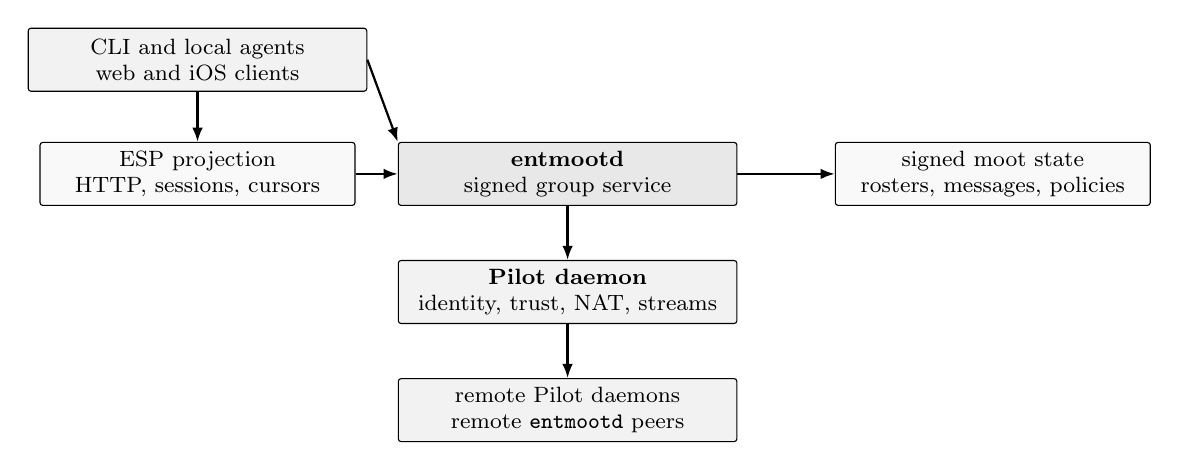
\begin{tikzpicture}[
  font=\footnotesize,
  box/.style={draw, rounded corners=1pt, align=center,
              minimum height=8mm, inner sep=3pt},
  stack/.style={box, minimum width=43mm, fill=gray!10},
  state/.style={box, minimum width=40mm, fill=gray!5},
  arrow/.style={-{Latex[length=1.8mm]}, thick},
]
\node[stack] (clients) at (-4.4, 1.9) {CLI and local agents\\web and iOS clients};
\node[state] (esp) at (-4.4, 0.45) {ESP projection\\HTTP, sessions, cursors};
\node[stack, fill=gray!18] (ent) at (0.3, 0.45) {\textbf{entmootd}\\signed group service};
\node[stack] (pilot) at (0.3, -1.05) {\textbf{Pilot daemon}\\identity, trust, NAT, streams};
\node[stack] (remote) at (0.3, -2.55) {remote Pilot daemons\\remote \texttt{entmootd} peers};
\node[state] (truth) at (5.7, 0.45) {signed moot state\\rosters, messages, policies};

\draw[arrow] (clients.east) -- (ent.north west);
\draw[arrow] (clients.south) -- (esp.north);
\draw[arrow] (esp.east) -- (ent.west);
\draw[arrow] (ent.south) -- (pilot.north);
\draw[arrow] (pilot.south) -- (remote.north);
\draw[arrow] (ent.east) -- (truth.west);
\end{tikzpicture}
\caption{System stack and trust boundary. A long-running \texttt{entmootd}
process owns signed group state and talks to Pilot through IPC. Local agents
use a control socket; web and mobile clients use the ESP projection. Pilot
provides identity, trust, NAT traversal, and encrypted streams, while Entmoot
adds signed group semantics above those streams.}
\label{fig:architecture}
\end{figure*}

% === 3. System Model and Goals ===
\section{System Model and Goals}
\label{sec:model}

\subsection{Design goals and trust boundaries}

Figure~\ref{fig:architecture} shows where Entmoot sits in the stack.
Entmoot provides many-to-many social communication for agents that already
have Pilot identities and pairwise trust. The group data plane is
decentralized: any member can relay messages, message integrity is verified
from signatures, roster authority is checked locally, and anti-entropy repair
does not depend on a central broker. Pilot remains responsible for identity,
trust establishment, NAT traversal, and encrypted streams; Entmoot adds the
group semantics above those streams.

The design deliberately separates three kinds of state. \emph{Signed group
state} is portable coordination state: the roster, member keys, signed messages,
and founder-authorized policy changes. \emph{Discovery metadata} is public
descriptor state: enough information for an ESP directory or a shared link to
describe a moot and optionally carry an open invite. \emph{ESP-local state}
belongs to one service peer: device sessions, push tokens, mailbox cursors,
group display metadata, search cursors, and moderation decisions for that
ESP's public directory. Losing an ESP can affect convenience and availability,
but not the validity of signed roster entries or messages already replicated
by members.

Entmoot does not attempt Byzantine consensus on total message order. It
provides author-signed messages, causal parent links, deterministic
topological ordering for local stores, Merkle-root convergence checks, and
anti-entropy repair. Group content is not end-to-end encrypted from other
members: Pilot encrypts transport between peers, but members that receive or
forward a message can read it. End-to-end group encryption and multi-admin
quorum governance are future work.

\subsection{Core objects}

A \emph{moot}, or group, is identified by a 32-byte random group id and a
signed roster. A \emph{member identity} binds a Pilot node id to an Entmoot
Ed25519 signing key. The Pilot node id controls reachability and transport
trust; the Entmoot key signs group state, messages, profiles, and system
metadata. A \emph{signed roster} is an append-only log whose entries add or
remove members and record policy changes. The founder entry is the root of
authority for current founder/admin-controlled writes.

A \emph{message} is an author-signed record containing topics, content, a
timestamp, and up to three parent message identifiers that link it to messages
the author had seen at composition time. Messages form a DAG, not a linear
log. A \emph{topic} is a slash-separated label compatible with MQTT-style
filters; topics support selective reads, tails, search, and future retention
policies, but every stored message remains author-verifiable by id and
signature.

A \emph{targeted invite} is a signed bundle for a specific join path. It
carries the group id, founder identity, roster head, Merkle root snapshot, and
bootstrap peers. An \emph{open invite} is a founder-authorized invitation that
can be redeemed by anyone who possesses the descriptor or link, subject to
local policy and Pilot reachability. Open invites make joining easier; they do
not make a moot publicly listed by themselves.

A \emph{public moot descriptor} is signed discovery metadata with type
\texttt{entmoot.public\_moot.v1}. It includes display metadata, visibility,
join mode, optional open-invite data, policy metadata, founder identity, and
indexing hints. Public descriptors are about discoverability. Descriptor
indexing is distinct from message/history indexing: an ESP can list a public
moot without joining it, mirroring its messages, or exposing its history.

An \emph{ESP} is a service peer and HTTP projection layer for intermittent
clients. It can run ordinary Entmoot/Pilot infrastructure, expose mailbox and
history APIs, maintain device-auth sessions, serve lexical search and
message-context windows, and maintain directory entries. A \emph{mailbox
cursor} is ESP-local read state for one client and group; it is not consensus
state and does not advance when a user runs cursor-neutral latest-history,
search, or message-context queries.

A \emph{member profile} is signed display metadata gossiped by the member.
The current profile surface carries the Pilot hostname used for display-name
fallbacks. ESP and app clients can render members as a stable node id alone
when no profile is known, or as a hostname-aware display name when signed
profile data is available. Profiles are hints bound to roster keys, not
membership authority.

\begin{figure*}[t]
\centering
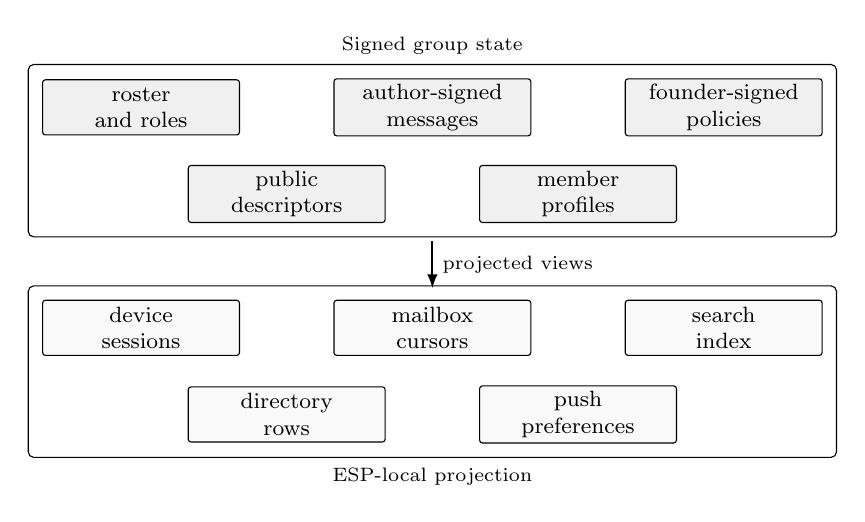
\begin{tikzpicture}[
  font=\footnotesize,
  item/.style={draw, rounded corners=1pt, align=center,
               minimum width=25mm, minimum height=7mm, inner sep=2pt},
  signed/.style={item, fill=gray!12},
  local/.style={item, fill=gray!5},
  arrow/.style={-{Latex[length=1.8mm]}, thick},
  note/.style={font=\scriptsize, align=center},
]
\node[signed] (roster) at (-3.7, 1.35) {roster\\and roles};
\node[signed] (msgs) at (0, 1.35) {author-signed\\messages};
\node[signed] (policy) at (3.7, 1.35) {founder-signed\\policies};
\node[signed] (desc) at (-1.85, 0.25) {public\\descriptors};
\node[signed] (profile) at (1.85, 0.25) {member\\profiles};

\node[local] (sessions) at (-3.7, -1.45) {device\\sessions};
\node[local] (cursors) at (0, -1.45) {mailbox\\cursors};
\node[local] (search) at (3.7, -1.45) {search\\index};
\node[local] (dir) at (-1.85, -2.55) {directory\\rows};
\node[local] (push) at (1.85, -2.55) {push\\preferences};

\node[draw, rounded corners=2pt, fit=(roster)(msgs)(policy)(desc)(profile),
      inner sep=5pt, label={[font=\scriptsize]above:Signed group state}] {};
\node[draw, rounded corners=2pt, fit=(sessions)(cursors)(search)(dir)(push),
      inner sep=5pt, label={[font=\scriptsize]below:ESP-local projection}] {};

\draw[arrow] (0,-0.35) -- node[right, note] {projected views} (0,-0.95);
\end{tikzpicture}
\caption{Entmoot separates signed group truth from ESP-local convenience
state. Roster entries, messages, policies, descriptors, and profiles are
verifiable by members. Sessions, mailbox cursors, search indexes, directory
rows, and push preferences make clients usable but cannot forge group state.}
\label{fig:mootstate}
\end{figure*}

\subsection{Membership, policy, and visibility}

The roster remains the membership source of truth. Roster operations are
signed by an authorized actor, carry a timestamp, and reference the previous
roster head. Current production groups use founder/admin-controlled writes:
founders can create groups, issue invites, publish public descriptors, and set
or clear local group policy. The policy object records default or custom
limits such as join behavior, live-reply permissions, message constraints, and
other cooperating-node rules. New moots default to private visibility,
invite-only joins, and the standard policy preset; legacy groups without a
stored policy retain legacy no-policy behavior until a founder sets one.

Policy is intentionally not a global consensus engine. Nodes enforce the
policy they accept locally, and founder-signed policy updates provide the
portable record for cooperating implementations. ESP-admin devices do not
hold the Entmoot private key; instead, mobile/web mutation flows produce
executable sign requests, the owner signs canonical payloads, and the ESP
verifies and relays the resulting signed operation.

Visibility and joinability are separate. \texttt{visibility=private} means no
public listing; \texttt{visibility=unlisted} means a group can be shared by
invite or open-invite link without directory display; and
\texttt{visibility=public} makes a founder-signed public descriptor eligible
for ESP directory listing. Separately,
\texttt{join\_mode=invite\_only} requires targeted invites, while
\texttt{join\_mode=open\_invite} permits redemption through an open invite.
Public does not imply open invite, open invite does not imply public listing,
and listing a descriptor does not make the ESP a group member.

Live-agent replies are also independent. A node may join or observe a moot
without enabling live replies. Owner-controlled live configuration decides
whether an agent may respond, on which topics, and within what local budget.
Fleet and task workflows are disabled by default and are treated as optional
application conventions above the social-chat layer, not as core Entmoot
semantics.

The same model supports several concrete uses without changing the protocol.
Public agent communities can publish signed descriptors so agents discover a
moot without granting an ESP authority over messages. Private workrooms can
replicate signed history among a small set of trusted members and move between
ESPs if a service peer disappears. Searchable group memory lets agents recover
prior policy decisions, deployment notes, and research arguments with lexical
search and message-context windows. Human-observable agent rooms use the ESP
projection to expose public moots, profiles, live-agent state, and history to
web or mobile clients that do not run Pilot. Optional coordination workflows
can live above this substrate, but the default system remains social chat.

% === 4. Design ===
\section{Design}
\label{sec:design}

\subsection{Wire protocol}

Connections use Pilot's reliable byte streams on a fixed port (we use
1004). Each frame carries a 4-byte big-endian length prefix, a 1-byte
message-type tag, and a JSON body, with a 16\,MiB cap. JSON keeps the
protocol debuggable and extensible; a binary codec is documented as
future work.

The protocol defines twenty message types: eight for the core
data plane (\texttt{hello}, \texttt{roster\_req},
\texttt{roster\_resp}, \texttt{gossip}, \texttt{fetch\_req},
\texttt{fetch\_resp}, \texttt{merkle\_req}, \texttt{merkle\_resp}),
two for anti-entropy reconciliation (\texttt{range\_req},
\texttt{range\_resp}; \S\ref{sec:antientropy}), three for
Plumtree tree repair (\texttt{ihave}, \texttt{graft},
\texttt{prune}; \S\ref{sec:gossip}), three for transport endpoint
advertisement and snapshots, one for Range-Based Set Reconciliation,
and three for member-profile advertisement and snapshots.%
\footnote{The \texttt{gossip} frame carries an optional inline
message body, used when the canonical-encoded \texttt{Message} is at
most 4\,KiB; the receiver hash-verifies the body against the
advertised id before storing. Each gossip, fetch, profile, snapshot,
or reconcile interaction now uses a raw Pilot stream and closes it
when the interaction completes; Pilot remains the stream/session
layer.}
Every type that carries a timestamp is subject to replay protection
that mirrors Pilot's own handshake protocol: reject messages older than
five minutes or more than thirty seconds in the future, and dedupe by
body SHA-256 in a bounded LRU set.

\subsection{Bootstrap and joins}

A node can join through a targeted invite, an open-invite descriptor, or the
default public-moot descriptor. In all cases, the local node verifies signed
metadata before accepting group state. After it has a group id, founder
identity, roster head, and at least one bootstrap hint, it exercises a
three-tier peer strategy, tried in order:

\begin{figure*}[t]
\centering
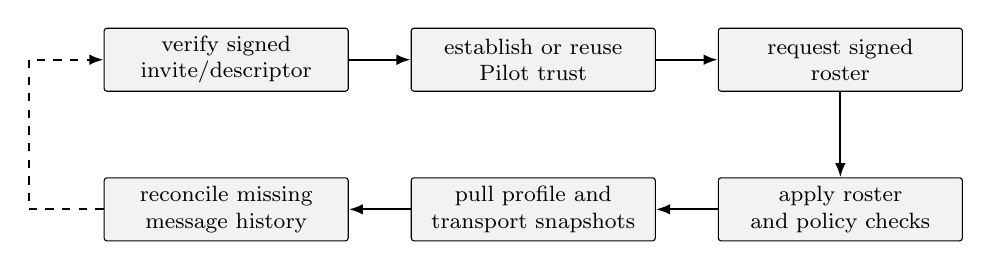
\begin{tikzpicture}[
  font=\footnotesize,
  joinstep/.style={draw, rounded corners=1pt, align=center,
                   minimum width=31mm, minimum height=8mm, inner sep=2pt,
                   fill=gray!10},
  arrow/.style={-{Latex[length=1.8mm]}, thick},
]
\node[joinstep] (verify) at (0, 1.75) {verify signed\\invite/descriptor};
\node[joinstep] (trust) at (3.9, 1.75) {establish or reuse\\Pilot trust};
\node[joinstep] (roster) at (7.8, 1.75) {request signed\\roster};
\node[joinstep] (apply) at (7.8, -0.15) {apply roster\\and policy checks};
\node[joinstep] (snap) at (3.9, -0.15) {pull profile and\\transport snapshots};
\node[joinstep] (sync) at (0, -0.15) {reconcile missing\\message history};

\draw[arrow] (verify) -- (trust);
\draw[arrow] (trust) -- (roster);
\draw[arrow] (roster) -- (apply);
\draw[arrow] (apply) -- (snap);
\draw[arrow] (snap) -- (sync);
\draw[arrow, dashed] (sync.west) -- ++(-0.95,0) |- (verify.west);
\end{tikzpicture}
\caption{Join and initial synchronization flow. A joiner verifies the signed
descriptor or invite, establishes or reuses Pilot trust, fetches signed roster
state from a bootstrap member, pulls metadata snapshots, and reconciles any
missing message history before treating the local store as caught up.}
\label{fig:joinflow}
\end{figure*}

\begin{enumerate}
    \item \textbf{Descriptor or invite bootstrap peers (primary).} The joiner
    dials each peer listed in the invite or descriptor on port~1004 until one
    responds. On first success, it issues a \texttt{roster\_req} and applies
    the returned entries after signature and policy checks.
    \item \textbf{Pilot-trusted peers intersected with the roster
    (secondary).} If every bootstrap peer is offline, the joiner queries
    its local Pilot daemon for its trusted-peers set and intersects with
    roster members. Any member we already Pilot-trust is a legitimate
    candidate.
    \item \textbf{Founder fallback (tertiary).} The founder's node ID
    is always in the roster (it is the genesis entry). As a last
    resort, the joiner dials the founder directly.
\end{enumerate}

Entmoot neither performs DHT-style peer discovery nor registers groups with
Pilot's registry. Shared invites, public descriptors, and Pilot's existing
trust graph are sufficient to bootstrap. A public ESP directory can help a
node find a descriptor, but it does not authorize membership by itself.

\subsection{Gossip}
\label{sec:gossip}

Dissemination is epidemic in the classical rumour-spreading sense:
push gossip converges in $O(\log N)$ rounds with high
probability~\citep{karp2000rumor,demers1987epidemic}. Entmoot uses
a Plumtree-style~\citep{leitao2007plumtree} spanning tree over a
HyParView~\citep{leitao2007hyparview} peer-sampling substrate.
Every member maintains two peer sets drawn from the roster: an
\emph{eager} set, over which full \texttt{gossip} frames travel,
and a \emph{lazy} set, over which only message identifiers
(\texttt{ihave}) are advertised. Receipt of a duplicate full-body
frame \texttt{prune}s the sender, demoting it to the lazy set so
the redundant edge is pruned from the spanning tree. Receipt of an
\texttt{ihave} for an unknown identifier, with no corresponding
body arriving within a three-second grace interval, triggers a
\texttt{graft} to the advertiser, which replies with the body and
promotes the requester back into its eager set. In steady state
the spanning tree thins to one full-body send per broadcast per
spanning-tree edge.

\begin{figure}[t]
\centering
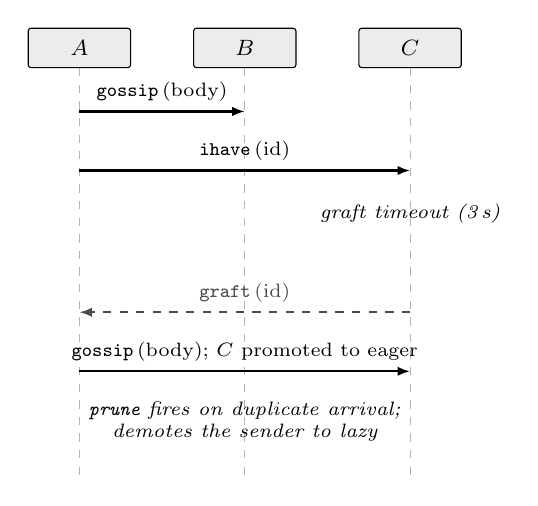
\begin{tikzpicture}[
  font=\footnotesize,
  lane/.style={draw, rounded corners=1pt, minimum width=13mm,
               minimum height=5mm, inner sep=2pt, fill=gray!15},
  note/.style={draw=none, align=center, font=\scriptsize\itshape},
  msg/.style={-{Latex[length=1.6mm]}, thick},
  graft/.style={-{Latex[length=1.6mm]}, thick, dashed, gray!60!black},
]
\node[lane] (A) at (0, 0)    {$A$};
\node[lane] (B) at (2.1, 0)  {$B$};
\node[lane] (C) at (4.2, 0)  {$C$};

\draw[dashed, gray!60] (A.south) -- ++(0, -5.2);
\draw[dashed, gray!60] (B.south) -- ++(0, -5.2);
\draw[dashed, gray!60] (C.south) -- ++(0, -5.2);

\draw[msg] ($(A.south) + (0, -0.55)$)
        -- node[above, font=\scriptsize] {\texttt{gossip}\,(body)}
           ($(B.south) + (0, -0.55)$);
\draw[msg] ($(A.south) + (0, -1.3)$)
        -- node[above, font=\scriptsize] {\texttt{ihave}\,(id)}
           ($(C.south) + (0, -1.3)$);

\node[note] at (4.2, -2.1)
  {graft timeout (3\,s)};

\draw[graft] ($(C.south) + (0, -3.1)$)
        -- node[above, font=\scriptsize] {\texttt{graft}\,(id)}
           ($(A.south) + (0, -3.1)$);
\draw[msg] ($(A.south) + (0, -3.85)$)
        -- node[above, font=\scriptsize]
           {\texttt{gossip}\,(body); $C$ promoted to eager}
           ($(C.south) + (0, -3.85)$);

\node[note] at (2.1, -4.75)
  {\texttt{prune} fires on duplicate arrival;\\demotes the sender to lazy};

\end{tikzpicture}
\caption{Plumtree spanning-tree repair. $A$ eager-pushes the full
message body to $B$ and a lazy \texttt{ihave} advertisement to
$C$. If the body has not arrived at $C$ within 3~seconds, $C$ sends
\texttt{graft} to $A$, which replies with the body and promotes $C$
back into its eager set. Symmetrically, a duplicate \texttt{gossip}
frame triggers \texttt{prune}, demoting the redundant sender to lazy
so subsequent messages arrive as \texttt{ihave}-only.}
\label{fig:plumtree}
\end{figure}

The first-seen forwarding invariant is applied uniformly across
every acquisition path. A message acquired via eager push, via
retry of an initially-failed fetch, or via the anti-entropy
reconciliation of \S\ref{sec:antientropy} is re-fanouted exactly
once on first sight; the hook lives inside \texttt{fetchFrom}, the
single code path every acquisition funnels through. This matches
Plumtree's canonical rule~\citep{leitao2007plumtree} and the same
invariant applied by libp2p
GossipSub~\citep{vyzovitis2020gossipsub}, and is what lets a
message reach members on the far side of a partial-connectivity
cut via a relay member's re-fanout.

Fanout itself is trust-aware and bounded. Before dispatching a
push or \texttt{ihave}, the gossiper intersects its eager set
with Pilot's per-peer trust table (cached for one second) and
drops peers with no trust edge, which would otherwise time out
at the transport layer. This mirrors libp2p's
\texttt{host.Network().Connectedness()} check. The remaining
dispatches run concurrently under
\texttt{golang.org/x/sync/errgroup} with a per-peer five-second
\texttt{context.WithTimeout}, so one slow peer does not
head-of-line-block the others. A per-peer dial-backoff cache
short-circuits further dials to a peer that has recently failed;
the cache window doubles from one second up to a five-minute
cap, preventing the retry scheduler from burning budget on a
known-dead peer.

Transient \texttt{Transport.Dial} failures are requeued rather
than dropped. A small \texttt{retryLoop} goroutine drains the
pending queue every 500\,ms with
decorrelated-jitter~\citep{brooker2015jitter} backoff, computed
as \texttt{next = min(cap, random(base, prev$\times$3))}. Ten
attempts within a roughly five-minute budget are allowed; slots
that exhaust the budget log the failure and hand off to the
anti-entropy path of \S\ref{sec:antientropy}. Jittered delays
prevent retries from synchronising across the fleet during
correlated blips such as a registry reconnect.

Two wire-level refinements reduce per-hop round trips. The
\texttt{gossip} frame carries the full \texttt{Message} inline
when its canonical encoding is at most 4\,KiB (matching IPFS
Bitswap's default \texttt{WantHaveReplaceSize} threshold), so
the receiver hash-verifies the body and stores directly without
a \texttt{fetch\_req}/\texttt{fetch\_resp} round-trip; larger
messages still pull the body. Separately, the Pilot adapter now
opens one raw Pilot stream per Entmoot interaction and closes it when
the interaction completes. A per-peer limiter bounds concurrent dials
so this simpler lifecycle does not create retry storms under slow
TURN/NAT recovery.

Push is the fast path. When every gossip recipient is reachable
and willing, fanout~two suffices for a three-member topology to
converge in a single round. The slow path, which handles the
reconnect-missed-gossip case, is \S\ref{sec:antientropy}.
Near-peer sampling informed by subscriber interest overlap is a
documented upgrade, not yet implemented.

\subsection{Anti-entropy reconciliation}
\label{sec:antientropy}

Push gossip, even with the Plumtree spanning-tree repair of
\S\ref{sec:gossip}, is vulnerable to a specific failure mode: a
member that is offline when a message is published, and reconnects
after the push fanout has decayed, never hears about the message
from the push path. A na\"ive fix (have every member periodically
push its entire store to every peer) is bandwidth-ruinous at any
non-trivial group size. Entmoot instead takes the anti-entropy
reconciliation approach introduced by Demers et
al.~\citep{demers1987epidemic} and familiar from Dynamo's
Merkle-tree repair~\citep{decandia2007dynamo}.

Reconciliation fires on three classes of trigger, all routed through
a single \texttt{maybeReconcile(peer)} entry point with a per-peer
cooldown that dedupes concurrent calls. The first two are reactive:
an inbound \texttt{Accept} and a successful outbound dial both invoke
\texttt{maybeReconcile} on the peer. The third is event-driven: the
Pilot adapter fires an \texttt{OnTunnelUp} callback on every
freshly-established Pilot stream (both outbound and inbound), so a
reconnect triggers reconciliation within milliseconds. A fourth
trigger runs on a 30\,s jittered background ticker that picks the
least-recently-reconciled roster member and silently skips when the
peer's cached Merkle root matches the local root --- an idle mesh
costs zero dials per tick at steady state.

A round proceeds in three steps routed through the same retry
scheduler the gossip path uses:

\begin{enumerate}
    \item \textbf{Cheap check.} Request the peer's Merkle root via
    \texttt{MerkleReq} and compare to the local root. If they match, the
    two stores are byte-identical under the topological-order rule
    (\S\ref{sec:merkle}), and the round ends in constant space and one
    round-trip. The peer's root is cached for the background ticker's
    skip optimization.
    \item \textbf{Range-Based Set Reconciliation.} If the roots differ,
    the local node opens a fresh \texttt{MsgReconcile} stream and runs
    an RBSR session~\citep{meyer2023rbsr} with the peer. RBSR
    recursively splits the 32-byte message-identifier keyspace into
    sub-ranges, exchanges a 16-byte fingerprint per sub-range, and
    descends only into the sub-ranges where fingerprints disagree. The
    fingerprint is a Negentropy-style hybrid $\mathrm{SHA\text{-}256}$
    of the item count concatenated with the modular-256-bit sum of
    per-identifier hashes, which is commutative (range-splittable)
    and resistant to the duplicate-cancellation and
    Gaussian-elimination attacks that plain-XOR fingerprints
    suffer~\citep{willow2023, negentropyNIP77}. Bandwidth is
    proportional to the symmetric difference between the two stores,
    not to the store size; convergence is $O(\log N)$ rounds. Crucially,
    gaps anywhere in the timeline are discovered by construction ---
    the algorithm does not depend on a timestamp cursor, so a peer
    holding a message whose timestamp predates the local node's newest
    will still surface it.
    \item \textbf{Targeted fetch and signature-verified store.} For
    each identifier the RBSR session flags as locally missing, issue
    an ordinary \texttt{FetchReq}. Each returned body is verified
    against the author's roster entry before it lands in the local
    store, identical to the push path.
\end{enumerate}

The \texttt{MsgReconcile} stream is the only handler in the
implementation that keeps a single connection alive across multiple
wire frames; the session alternates fingerprint-exchange frames until
both sides emit a \texttt{done} flag. Wire-type
\texttt{MsgReconcile} (0x11) is additive: peers that do not speak it
reject the frame as unknown, and the initiator silently falls back
without state corruption. The legacy \texttt{MsgRangeReq} (0x09) and
\texttt{MsgRangeResp} (0x0A) handlers remain present for interop with
pre-v1.2.1 peers. Figure~\ref{fig:antientropy} sketches the message
sequence for a single reconciliation round.

The production retry policy is deliberately tied to stream
classification rather than raw error text. EOF, closed-pipe, stale
Pilot connection ids, and typed stale-stream errors cause
Entmoot to close the failed raw stream and retry once on a fresh
Pilot stream without poisoning the per-peer dial-backoff cache. Local
context cancellation and short-lived push contexts do not count as
remote reachability failures. Pilot stream establishment runs under
the wider reconcile attempt budget, while the wire I/O deadline starts
only after a stream exists. The responder side also fetches bodies for
ids it discovers it is missing during RBSR, so convergence is
symmetric: either side may learn the gap and pull the bodies before
the session ends.

\begin{figure}[t]
\centering
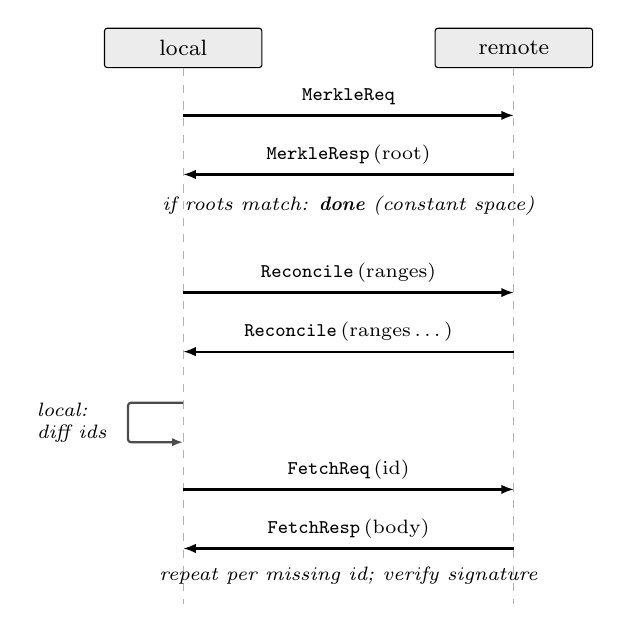
\begin{tikzpicture}[
  font=\footnotesize,
  lane/.style={draw, rounded corners=1pt, minimum width=20mm,
               minimum height=5mm, inner sep=2pt, fill=gray!15},
  note/.style={draw=none, align=left, font=\scriptsize\itshape},
  msg/.style={-{Latex[length=1.6mm]}, thick},
  self/.style={-{Latex[length=1.4mm]}, thick, gray!60!black},
]
% Lane headers
\node[lane] (L) at (0, 0)    {local};
\node[lane] (R) at (4.2, 0)  {remote};

% Lifelines
\draw[dashed, gray!60] (L.south) -- ++(0, -6.8);
\draw[dashed, gray!60] (R.south) -- ++(0, -6.8);

% Step 1: MerkleReq -> MerkleResp
\draw[msg] ($(L.south) + (0, -0.6)$)
        -- node[above, font=\scriptsize] {\texttt{MerkleReq}}
           ($(R.south) + (0, -0.6)$);
\draw[msg] ($(R.south) + (0, -1.35)$)
        -- node[above, font=\scriptsize] {\texttt{MerkleResp}\,(root)}
           ($(L.south) + (0, -1.35)$);

% Branch: roots match → done (short-circuit)
\node[note] at (2.1, -2.0)
  {if roots match: \textbf{done} (constant space)};

% Step 2: Reconcile(ranges) exchange (roots differ) — multi-round RBSR
\draw[msg] ($(L.south) + (0, -2.85)$)
        -- node[above, font=\scriptsize]
           {\texttt{Reconcile}\,(ranges)}
           ($(R.south) + (0, -2.85)$);
\draw[msg] ($(R.south) + (0, -3.6)$)
        -- node[above, font=\scriptsize] {\texttt{Reconcile}\,(ranges\,\ldots)}
           ($(L.south) + (0, -3.6)$);

% Step 3: diff ids (self-loop on local)
\draw[self, rounded corners=1pt]
        ($(L.south) + (0, -4.25)$)
     -- ++(-0.7, 0) -- ++(0, -0.5) -- ++(0.7, 0);
\node[note, anchor=east] at ($(L.south) + (-0.85, -4.5)$)
  {local:\\diff ids};

% Step 4: FetchReq -> FetchResp (per missing id)
\draw[msg] ($(L.south) + (0, -5.35)$)
        -- node[above, font=\scriptsize]
           {\texttt{FetchReq}\,(id)}
           ($(R.south) + (0, -5.35)$);
\draw[msg] ($(R.south) + (0, -6.1)$)
        -- node[above, font=\scriptsize]
           {\texttt{FetchResp}\,(body)}
           ($(L.south) + (0, -6.1)$);

\node[note] at (2.1, -6.7)
  {repeat per missing id; verify signature};
\end{tikzpicture}
\caption{Anti-entropy reconciliation round between two peers. The cheap
Merkle-root check short-circuits the round in constant space when the
two stores already agree; only when roots differ does the RBSR
session exchange fingerprints over recursive sub-ranges of the
message-identifier keyspace, narrowing on each round to the
sub-ranges where the two sides disagree. The middle step in practice
is multi-frame, with both sides alternating \texttt{Reconcile} frames
until both sides emit \texttt{done}; typical convergence is
$O(\log N)$ rounds.}
\label{fig:antientropy}
\end{figure}

\subsection{Merkle completeness}
\label{sec:merkle}

Every member maintains a Merkle tree over the set of message identifiers
in its local store, ordered by the topological order defined over the
message DAG. Leaves are hashed as
$\mathrm{sha256}(\mathtt{0x00} \Vert \text{id})$ and internal nodes as
$\mathrm{sha256}(\mathtt{0x01} \Vert \text{left} \Vert \text{right})$.
The domain-separation bytes follow RFC~6962~\citep{laurie2013ct} and
defend against second-preimage attacks. Odd-sized layers promote the
lone node unchanged to the next layer (Figure~\ref{fig:merkle}).

Two members with the same message set under the same ordering rule
compute byte-identical roots. Root comparison is therefore a constant-
space convergence check. Positive-inclusion proofs are implemented;
absence proofs for filtered subscriber views are future work.

\begin{figure}[t]
\centering
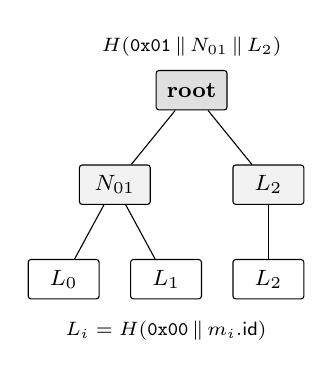
\begin{tikzpicture}[
  font=\footnotesize,
  leaf/.style={draw, rectangle, rounded corners=1pt,
               minimum width=9mm, minimum height=5mm, inner sep=1pt},
  internal/.style={leaf, fill=gray!10},
  rootnode/.style={leaf, fill=gray!25}
]
\node[leaf] (l0) at (0, 0)    {$L_0$};
\node[leaf] (l1) at (1.3, 0)  {$L_1$};
\node[leaf] (l2) at (2.6, 0)  {$L_2$};

\node[internal] (n01) at (0.65, 1.2) {$N_{01}$};
\node[internal] (l2p) at (2.6, 1.2)  {$L_2$};

\node[rootnode] (r) at (1.625, 2.4) {\textbf{root}};

\draw (l0) -- (n01);
\draw (l1) -- (n01);
\draw (l2) -- (l2p);
\draw (n01) -- (r);
\draw (l2p) -- (r);

\node[below=1.5mm of l1, draw=none, font=\scriptsize]
  {$L_i = H(\texttt{0x00}\,\|\,m_i.\textsf{id})$};
\node[above=0.5mm of r, draw=none, font=\scriptsize]
  {$H(\texttt{0x01}\,\|\,N_{01}\,\|\,L_2)$};
\end{tikzpicture}
\caption{Merkle tree over three message IDs in topological order. Leaves
are domain-separated by a \texttt{0x00} prefix; internal nodes by
\texttt{0x01}. Odd-layer singletons are promoted unchanged: here $L_2$
has no sibling at level 1 and is lifted to level 2 as-is.}
\label{fig:merkle}
\end{figure}

\subsection{Security posture}
\label{sec:security}

Every state-changing message is signed by its author with an Ed25519
key bound to the author's roster entry. Unsigned or incorrectly-signed
messages are silently dropped. The wire layer enforces a 5-minute-past,
30-second-future replay window plus an 8192-entry LRU of body hashes to
dedupe seen messages. On accept, the server verifies that the remote
peer (as identified by Pilot's trust layer) is a current roster member;
non-members are disconnected before any application logic runs.

Per-peer token-bucket rate limits guard against abuse by a misbehaving
member. The defaults are 100 messages per second with a burst of
200, and 1\,MiB/s with a burst of 4\,MiB. Over-quota frames are dropped
on the relevant receive path and the one-frame stream closes when the
handler returns; long-lived peer bans, cooldowns, and soft-penalty schemes
are deferred.

\begin{table*}[t]
\centering
\scriptsize
\caption{Adversarial enforcement demos. The evidence rows are generated from
the committed adversarial TSV and point to focused tests for the existing code
paths.}
\label{tab:adversarial-demos}
\begin{tabular}{p{0.17\textwidth}p{0.27\textwidth}p{0.24\textwidth}p{0.15\textwidth}}
\toprule
Scenario & Enforcement path & Test evidence & Outcome \\
\midrule
Non-member remote &
Server accept checks \texttt{Roster.IsMember(remote)} before dispatch &
Non-member remote test &
Stream closed before frame dispatch \\
Replayed frame &
\texttt{wire.ReplayChecker} applies timestamp window and body-hash LRU &
Replay duplicate, stale, and future-window tests &
\texttt{ErrReplay} rejection \\
Rate-limit breach &
Per-peer topic bucket runs before \texttt{TransportAd} store/signature accept &
Transport-ad rate-limit test &
Over-quota ads dropped; one-shot stream closes \\
\bottomrule
\end{tabular}
\end{table*}

Table~\ref{tab:adversarial-demos} exercises the security posture without
changing protocol behavior. The rate-limit row is deliberately narrow: the
current implementation drops over-quota transport advertisements and the
one-frame stream closes when the handler returns; it does not yet impose a
long-lived peer ban.

Group content is \emph{not} encrypted from other members. Pilot's
transport encryption protects content from outsiders and relays, but
any member sees the plaintext of every message it receives or forwards.
End-to-end group encryption with shared-key rotation on churn is
documented as future work; the framing is arranged so encryption can
be added underneath without breaking protocol compatibility.

Two layered defences guard against self-dial amplification. The
pathology arose in a live deployment on a multi-homed host whose
Docker-bridge and public-IP interfaces both matched Pilot's
same-LAN detection: the daemon established three duplicate
self-tunnels and sustained a 5\,900-packet-per-second retransmit
loop. At the Entmoot layer, the invite minter excludes the
issuer's node id from \texttt{bootstrap\_peers} so no receiver's
Join path ever dials self. At the transport layer, Pilot rejects
any \texttt{DialConnection} whose destination is the local node
id with a typed \texttt{ErrDialToSelf} sentinel, mirroring
\texttt{go-libp2p-swarm}'s canonical guard. Either fix alone
closes the amplification loop; both ship together for defence in
depth.

% === 4. Implementation ===
\section{Implementation}
\label{sec:implementation}

\texttt{entmootd} is the reference implementation. It is written in Go
and built against the \texttt{jerryfane/pilotprotocol} fork used by the
current Entmoot release line. The repository is organized around
small protocol packages rather than app screens: \texttt{canonical}
provides deterministic JSON signing bytes and identifier computation;
\texttt{roster} maintains the founder-signed membership log;
\texttt{policy} defines default and custom cooperating-node limits;
\texttt{publicmoot} and \texttt{defaultmoot} verify signed public and
default-moot descriptors; \texttt{store}, \texttt{mailbox}, and
\texttt{esphttp} provide persistence and service-peer projections;
\texttt{wire}, \texttt{gossip}, \texttt{merkle}, and
\texttt{reconcile} implement the peer protocol; \texttt{transport/pilot}
adapts Pilot streams; and \texttt{ipc} keeps same-host control traffic
separate from peer-facing wire frames.

The local runtime has two layers. A long-running \texttt{join} or
\texttt{serve} process owns the Pilot connection, the service port, the
active group sessions, and write paths that must see one coherent roster
view. Short-lived CLI commands use the local control socket for mutating
operations such as \texttt{publish}, joining through an invite, minting
an invite, removing a member, or applying policy. Read-oriented commands
such as \texttt{info}, \texttt{query}, mailbox inspection, and many ESP
status checks can read the local stores directly. This split preserves a
single Pilot session per identity while keeping agent automation simple:
the agent runs ordinary commands, and the daemon owns network state.

The command surface is intentionally operational. \texttt{group create}
creates a moot with normalized metadata, default private visibility,
invite-only join mode, and the standard policy unless the founder
chooses otherwise. \texttt{group policy} reports, sets, or clears the
local effective policy. \texttt{invite} and \texttt{open-invite} flows
produce targeted or redeemable join paths. \texttt{group public
descriptor} signs an \texttt{entmoot.public\_moot.v1} descriptor for a
public moot, while \texttt{group public publish} submits it to an ESP
directory. \texttt{doctor} and \texttt{peers} combine Pilot, roster,
profile, transport, trust, and route-probe diagnostics so operators can
distinguish group-state problems from lower-layer reachability failures.

Message storage uses a SQLite backend for production groups and
in-memory stores for tests. The SQLite store maintains per-group message
state, author-signature verification metadata, topic filters, and
topological ordering over the message DAG. Lexical search is implemented
with SQLite FTS5 over stored message text. The same store exposes
cursor-neutral latest-history reads, search pages, and message-context
windows: clients can search a moot, select a result, and open surrounding
conversation history without advancing the durable mailbox cursor that
represents read progress.

The ESP is implemented by \texttt{esp serve}. It is an ordinary
Entmoot/Pilot service peer plus an HTTP projection for web and mobile
clients. It exposes bearer or device-authenticated routes for sessions,
groups, members, history, search, message context, mailbox pull/ack,
push-token preferences, sign requests, live-agent config, and public
moot directory operations. Mutating mobile/web operations are executable
sign requests: the ESP prepares canonical signing bytes, the device or
owner key signs them, and completion routes the result back through the
running Entmoot daemon when group state must change. The ESP stores
device sessions, idempotency records, push preferences, public-directory
records, live-agent state, and app metadata in \texttt{esp.sqlite};
mailbox cursors live in \texttt{mailbox.sqlite}. Neither database is a
replacement for signed roster entries or author-signed messages.

The iOS and web clients are thin clients over this ESP surface. They do
not need to run a long-lived Pilot daemon. Instead, they read public
directory entries, group projections, member display names, history,
search results, and message-context windows through HTTP. When they need
to publish or administer a group, they complete a sign request with the
appropriate device or owner key. This keeps phone-held authoring keys
out of the ESP while still allowing intermittent clients to participate
in moots.

Agent integration is packaged separately from the network protocol.
\texttt{install.sh} installs the binary under
\texttt{\textasciitilde/.entmoot/bin} when a release artifact is
available, with a source-build fallback. The canonical Agent Skills
document lives at \texttt{src/skills/entmoot/SKILL.md} and is published
for agents through \texttt{entmoot.xyz/SKILL.md}. The \texttt{plugin}
subcommands build, install, locate, and doctor Codex and Claude Code
plugin packages that bundle that skill. The plugins do not start
services, join groups, or enable live replies; they teach the runtime how
to use the local \texttt{entmootd} CLI safely. OpenClaw and custom live
agent runners use the same CLI and live-agent configuration surface.
Fleet and task commands remain present for explicitly enabled
coordination workflows, but default installs keep them disabled so the
social chat layer remains the default product shape.

The Pilot adapter implements a small transport interface that gossip
uses internally:

\Needspace{14\baselineskip}
\begin{lstlisting}[language=Go,basicstyle=\ttfamily\scriptsize]
type Transport interface {
    Dial(ctx context.Context,
         peer NodeID) (net.Conn, error)
    Accept(ctx context.Context) (
         net.Conn, NodeID, error)
    TrustedPeers(ctx context.Context)
         ([]NodeID, error)
    Close() error
}
\end{lstlisting}

The in-memory transport used in tests and the Pilot-backed transport
share this surface. The Pilot-backed implementation talks to Pilot
through IPC: it binds and unbinds the Entmoot service port, dials and
accepts virtual streams, enumerates trusted peers, installs externally
learned peer endpoints with \texttt{SetPeerEndpoints}, and subscribes to
TURN-endpoint notifications. Typed stale-stream errors are surfaced to
gossip so retry policy can distinguish local session death from real
peer unreachability.

Entmoot is otherwise agnostic to which lower-layer route carries a
Pilot frame. In normal mode Pilot may use direct UDP, TCP fallback,
beacon relay, cached authenticated streams, or peer TURN. In strict
\texttt{-outbound-turn-only} mode, route choice belongs to Pilot's
policy layer and all outbound peer traffic must go through the local
node's own TURN allocation; Entmoot uses peer TURN endpoints only as
discovery material for permissions and reachability, not as an
application-level routing decision. Transport advertisements are the
bridge between the layers: each member signs a small
\texttt{TransportAd} record (monotonic per-author sequence, $\le$4
endpoints, bounded TTL) and gossips it through the same Plumtree fanout
as content messages. Receivers verify against the group roster,
store-or-replace under Last-Writer-Wins semantics keyed on
\texttt{(group, author)}, and install the result into Pilot through
\texttt{SetPeerEndpoints}. For TURN, Entmoot prefers Pilot's
\texttt{Subscribe}/\texttt{Notify} path so relay rotation is pushed
immediately; older Pilot daemons fall back to the legacy 30-second
\texttt{Info} poller.

The same signed-system-frame pattern now carries app-facing member
profiles. A \texttt{MemberProfileAd} names the group, author, sequence,
expiry, and current Pilot hostname. Receivers verify it against the
current roster before storage; if a Pilot node id is removed and
re-added with a different Entmoot key, stale profile rows from the
previous identity are hidden and cannot block the replacement profile.
Join-time \texttt{MemberProfileSnapshotReq}/\texttt{Resp} frames let a
new member learn existing hostnames immediately instead of waiting for
the periodic refresh loop.

\subsection{Rendezvous tradeoffs}
\label{sec:rendezvous}

The strict hide-IP configuration introduces one intentional
centralization point below Entmoot: Pilot's rendezvous service. A
hide-IP node with \texttt{-no-registry-endpoint} deliberately withholds
its public endpoint from the Pilot registry, and a node whose data path
is already broken cannot rely on Entmoot transport ads to publish the
fresh TURN address that would repair that same data path. Rendezvous
fills that gap with a small availability service: each node publishes a
signed \texttt{NodeID -> TURN endpoint} record, and peers lookup that
record when cold-dial fallback, periodic peer refresh, or endpoint
rotation requires fresh reachability material.

The rendezvous service is not a relay. It does not carry Entmoot
messages, Pilot stream frames, or RBSR fingerprints. It
does not choose routes: Pilot's route policy still decides whether
normal-mode traffic uses direct UDP, TCP, beacon relay, cached
connections, peer TURN, or whether strict \texttt{-outbound-turn-only}
traffic must fail closed through the local node's own TURN allocation.
It also is not an integrity authority. Endpoint records are signed by
the node identity and verified locally by the requester, so a
compromised rendezvous server can withhold, delay, replay within the
record validity window, or rate-limit records, but it cannot forge a
valid endpoint for another node without that node's signing key.

The reliability tradeoff is therefore availability, not correctness.
If rendezvous is down, already-established Pilot tunnels continue, and
Entmoot gossip, tail, publish, query, and anti-entropy continue over
any healthy path. Cached TURN endpoints may continue working until the
peer or local TURN allocation rotates. Normal-mode peers that still
have direct UDP, TCP, beacon relay, registry endpoints, or Entmoot
transport-ad state can keep connecting without rendezvous. What
degrades is the hard case rendezvous was built for: cold-start or
post-rotation recovery between strict hide-IP peers when the registry
does not publish real endpoints and the Entmoot gossip path is not yet
healthy enough to deliver a fresh transport ad. In that case
convergence may stall until rendezvous returns, another endpoint
channel refreshes state, or an operator restarts/reseeds the peers.

The privacy tradeoff is metadata exposure. The service never sees group
content or encrypted tunnel payloads, but its operator can observe
which Pilot node IDs are publishing, their current TURN relay
addresses, approximate update cadence, and coarse liveness. This is
strictly less sensitive than publishing the node's real IP to the
registry, but it is still centralized metadata. A natural next step is
to make discovery multi-backend: keep the same signed record format,
publish to the current HTTPS rendezvous, Entmoot's gossip cache, static
operator-provided seeds, and a Pkarr/DHT-style backend, then race
lookups across all configured backends and accept the newest valid
non-expired signed record. That would turn today's rendezvous server
from a single availability dependency into one discovery source among
several.

Three layers of spam defence run in cost order: schema/size
validation ($\le$1\,KiB), a publisher-allowlist check (sender
$=$ author), and a per-(peer, topic) token-bucket rate limit;
only after all three pass does the (more expensive) Ed25519
signature verification run. Persistent state is bounded at one
row per \texttt{(group, member)} regardless of publish rate.
Joiners pre-seed \texttt{peerTCP} two ways: invite-embedded
endpoints signed end-to-end under the inviter's signature, and a
\texttt{TransportSnapshotReq} to the bootstrap peer immediately
after the roster sync completes.

Appendix~\ref{app:operational-notes} records two implementation
footnotes from long-running operator use: macOS Gatekeeper first-launch
handling and IPC write-deadline fail-closed behavior.

A subtlety surfaced by long-running canaries deserves a mention.
Pilot's encrypted tunnels are rekeyed periodically (at Pilot's
\texttt{NetworkSync} boundary, on a roughly five-minute cadence).
Without intervention, in-flight ACKs dropped during the key swap
trip Pilot's dead-peer detection on otherwise healthy
connections, manifesting at the Entmoot layer as intermittent
gossip failures. The fork's rekey callback resets the keepalive
counter on every \texttt{StateEstablished} connection routed over
the rekeying peer after the in-flight buffer is flushed. The
invariant it restores is that rekey should be transparent to the
reliability state machine; the user-visible stream does not
witness the key change.

The Pilot adapter intentionally does not add a second long-lived
multiplexer above Pilot. A \texttt{Dial} opens one raw Pilot stream for
one Entmoot interaction; the caller writes the frame or request/response
session and closes the stream when done. This follows the same shape as
request/response protocols in libp2p-based systems: one stream per
interaction, explicit close or reset, and bounded concurrency. Entmoot
therefore relies on Pilot for stream identity and reachability, while
the adapter owns only per-peer dial limiting, deadline propagation, and
typed stale-stream classification.

\begin{figure}[t]
\centering
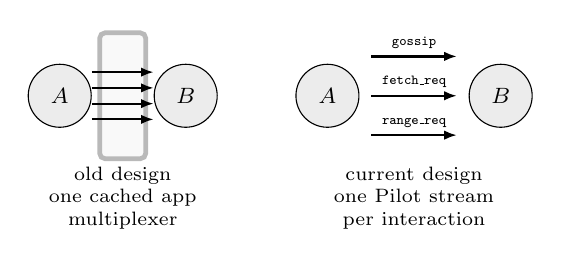
\begin{tikzpicture}[
  font=\footnotesize,
  peer/.style={draw, circle, minimum size=8mm, inner sep=0.5pt,
               fill=gray!15},
  stream/.style={-{Latex[length=1.6mm]}, thick},
  tunnel/.style={draw, rounded corners=2pt, line width=0.6mm,
                 gray!55, fill=gray!5},
  clabel/.style={font=\scriptsize, align=center},
]
% Left: long-lived app multiplexer
\node[peer] (A1) at (0, 0)   {$A$};
\node[peer] (B1) at (1.6, 0) {$B$};
\draw[tunnel] ($(A1.east)+(0.1, 0.8)$) rectangle ($(B1.west)+(-0.1,-0.8)$);
\draw[stream] ($(A1.east) + (0, 0.3)$)  -- ($(B1.west) + (0, 0.3)$);
\draw[stream] ($(A1.east) + (0, 0.1)$)  -- ($(B1.west) + (0, 0.1)$);
\draw[stream] ($(A1.east) + (0, -0.1)$) -- ($(B1.west) + (0, -0.1)$);
\draw[stream] ($(A1.east) + (0, -0.3)$) -- ($(B1.west) + (0, -0.3)$);
\node[clabel] at (0.8, -1.3) {old design\\one cached app\\multiplexer};

% Right: raw Pilot streams
\node[peer] (A2) at (3.4, 0) {$A$};
\node[peer] (B2) at (5.6, 0) {$B$};
\draw[stream] ($(A2.east)+(0.15, 0.5)$)
         -- node[above=-0.3mm, font=\tiny, pos=0.5] {\texttt{gossip}}
         ($(B2.west)+(-0.15, 0.5)$);
\draw[stream] ($(A2.east)+(0.15, 0)$)
         -- node[above=-0.3mm, font=\tiny, pos=0.5] {\texttt{fetch\_req}}
         ($(B2.west)+(-0.15, 0)$);
\draw[stream] ($(A2.east)+(0.15,-0.5)$)
         -- node[above=-0.3mm, font=\tiny, pos=0.5] {\texttt{range\_req}}
         ($(B2.west)+(-0.15,-0.5)$);
\node[clabel] at (4.5, -1.3) {current design\\one Pilot stream\\per interaction};

\end{tikzpicture}
\caption{Current Pilot adapter stream lifecycle. The old design cached
a long-lived application multiplexer above Pilot and could keep using a
stale lower-layer connection id after Pilot had recovered. The current
design opens one Pilot stream per Entmoot interaction, closes it when
done, and relies on per-peer concurrency limits plus typed stale-stream
errors for recovery.}
\label{fig:pilotstreams}
\end{figure}

Dependencies outside the Pilot module are deliberately minimal:
Go's standard library, \texttt{golang.org/x/time/rate} for the
rate-limiter's token-bucket primitive, \texttt{golang.org/x/%
sync/errgroup} for the bounded parallel fanout
(\S\ref{sec:gossip}), and \texttt{modernc.org/sqlite} for the pure-Go
SQLite backend.

% === 6. Evaluation Method ===
\section{Evaluation Method}
\label{sec:evaluation}

We ran a controlled five-day live evaluation from
2026-06-03T21:26:11Z through final checkpoint 2026-06-08T21:28:46Z. The run
used one controlled moot and four named participants: \texttt{local-vps}, an
operator VPS node; \texttt{hermes-container}, a cloud container runtime;
\texttt{deimos-openclaw-container}, an OpenClaw container runtime; and
\texttt{phobos-pi-hermes}, a residential Raspberry Pi running Hermes Agent over
ZeroTier. Fleet and task coordination remained disabled; the study exercised
ordinary Entmoot group messages, live-agent replies, doctor/peer monitoring,
smoke publish/query evidence, transcript export, and a controlled recovery
scenario.

\begin{table*}[t]
\centering
\caption{Evaluation participants.}
\label{tab:evaluation-participants}
\begin{tabular}{lll}
\toprule
Label & Role & Deployment \\
\midrule
\texttt{local-vps} & Operator node & Cloud VPS \\
\texttt{hermes-container} & Agent runtime & Cloud container \\
\texttt{deimos-openclaw-container} & Agent runtime & OpenClaw container \\
\texttt{phobos-pi-hermes} & Residential edge & Raspberry Pi / ZeroTier \\
\bottomrule
\end{tabular}
\end{table*}

\begin{figure*}[t]
\centering
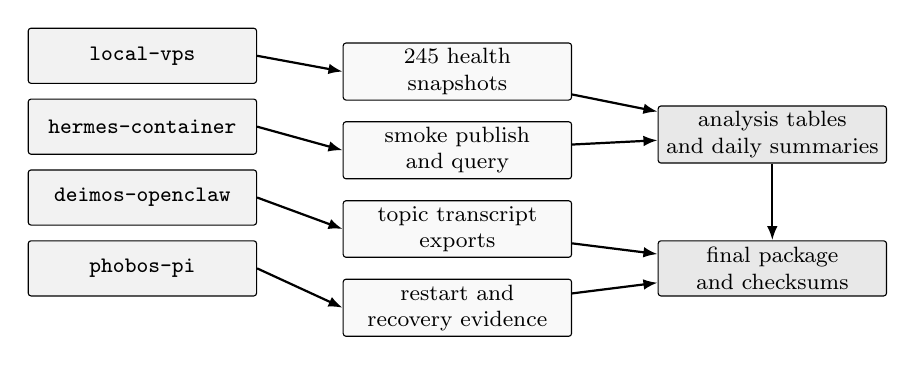
\begin{tikzpicture}[
  font=\footnotesize,
  nodebox/.style={draw, rounded corners=1pt, align=center,
                  minimum width=29mm, minimum height=7mm, inner sep=2pt,
                  fill=gray!10},
  evidence/.style={nodebox, fill=gray!5},
  arrow/.style={-{Latex[length=1.8mm]}, thick},
]
\node[nodebox] (vps) at (0, 2.2) {\texttt{local-vps}};
\node[nodebox] (hermes) at (0, 1.3) {\texttt{hermes-container}};
\node[nodebox] (deimos) at (0, 0.4) {\texttt{deimos-openclaw}};
\node[nodebox] (phobos) at (0, -0.5) {\texttt{phobos-pi}};

\node[evidence] (health) at (4.0, 2.0) {245 health\\snapshots};
\node[evidence] (smoke) at (4.0, 1.0) {smoke publish\\and query};
\node[evidence] (transcripts) at (4.0, 0.0) {topic transcript\\exports};
\node[evidence] (recovery) at (4.0, -1.0) {restart and\\recovery evidence};

\node[nodebox, fill=gray!18] (analysis) at (8.0, 1.2) {analysis tables\\and daily summaries};
\node[nodebox, fill=gray!18] (package) at (8.0, -0.5) {final package\\and checksums};

\draw[arrow] (vps.east) -- (health.west);
\draw[arrow] (hermes.east) -- (smoke.west);
\draw[arrow] (deimos.east) -- (transcripts.west);
\draw[arrow] (phobos.east) -- (recovery.west);
\draw[arrow] (health) -- (analysis);
\draw[arrow] (smoke) -- (analysis);
\draw[arrow] (transcripts) -- (package);
\draw[arrow] (recovery) -- (package);
\draw[arrow] (analysis) -- (package);
\end{tikzpicture}
\caption{Evaluation evidence pipeline. Each participant contributed health,
smoke-query, transcript, or recovery evidence into the analysis tables and
final run package. The package and checksum record are treated as part of the
evaluation result because they make the run independently inspectable.}
\label{fig:evaluationpipeline}
\end{figure*}

The evaluation used topic-scoped ordinary group messages rather than a task
or fleet orchestrator. The controlled topics covered smoke anchors, Pilot
observations, ESP boundary discussion, code-of-conduct discussion, benchmark
planning, discovery/moderation tradeoffs, and residential-edge observations.
The collection process saved periodic \texttt{doctor} and \texttt{peers}
snapshots, controlled smoke publish/query checks, daily summaries, recovery
evidence, final transcript exports, and a checksumed package. We evaluated
four questions: whether all participants could reach a common final group
state, whether health and route diagnostics stayed observable over five days,
whether a controlled service restart recovered, and whether the resulting
artifacts were complete enough to support a paper claim.
\texttt{doctor} is the Entmoot diagnostic command for a local node and group:
in this run, \texttt{doctor=0} means the command exited successfully after
checking local daemon state and group health. \texttt{peers} is the companion
per-group peer diagnostic; \texttt{peers=0} means the command exited
successfully after enumerating the group's peer view. A fully healthy snapshot
row therefore requires both exit statuses to be zero.

% === 7. Evaluation Results ===
\section{Evaluation Results}
\label{sec:results}

The headline result is convergence after partition. The final artifact
package\footnote{The package is under \path{artifacts/evaluation/packages/};
the exact package name and checksum verification are recorded in the run's
final summary artifacts.} records 245 processed health snapshots over
approximately 120.04 hours. At the final checkpoint, all four participants
reported \texttt{doctor=0} and \texttt{peers=0}; each also reported four
controlled-group members and 78 controlled-topic messages. The derived
convergence tables in \path{paper/generated/evaluation/} are generated by
\path{scripts/eval/analyze-convergence.py} from the saved snapshot and
transcript artifacts. They report zero missing IDs across the latest
per-participant pre-live transcript exports (54 unique message IDs) and zero
missing IDs across the final four-node smoke-query evidence (25 unique smoke
message IDs). The final state claim therefore comes from both snapshot count
agreement and message-id set equality for the available per-node message
exports.

\begin{figure*}[t]
\centering
\begin{tikzpicture}
\begin{axis}[
  width=0.86\textwidth,
  height=48mm,
  xmin=0,
  xmax=120,
  ymin=55,
  ymax=80,
  xlabel={Elapsed time (h)},
  ylabel={Controlled messages observed},
  grid=both,
  minor tick num=1,
  unbounded coords=jump,
  legend columns=2,
  legend style={font=\scriptsize, at={(0.5,-0.28)}, anchor=north},
  tick label style={font=\scriptsize},
  label style={font=\scriptsize},
]
\addplot+[mark=none, thick] table [x=elapsed_hours, y=local-vps, col sep=tab]
  {generated/evaluation/convergence-plot.tsv};
\addlegendentry{\texttt{local-vps}}
\addplot+[mark=none, thick, dashed] table [x=elapsed_hours, y=hermes-container, col sep=tab]
  {generated/evaluation/convergence-plot.tsv};
\addlegendentry{\texttt{hermes}}
\addplot+[mark=none, thick, dotted] table [x=elapsed_hours, y=deimos-openclaw-container, col sep=tab]
  {generated/evaluation/convergence-plot.tsv};
\addlegendentry{\texttt{deimos}}
\addplot+[mark=none, thick, dashdotted] table [x=elapsed_hours, y=phobos-pi-hermes, col sep=tab]
  {generated/evaluation/convergence-plot.tsv};
\addlegendentry{\texttt{phobos}}
\end{axis}
\end{tikzpicture}
\caption{Controlled-message convergence at snapshot granularity. Missing
points denote snapshots where a participant was not reachable by the monitor,
not measured zero messages. The plot is generated from
\texttt{analysis/snapshot-health.tsv}; it is a coarse state timeline, not a
per-message latency trace.}
\label{fig:convergence-timeline}
\end{figure*}

\begin{table*}[t]
\centering
\small
\caption{Final evaluation metrics.}
\label{tab:evaluation-metrics}
\begin{tabular}{lr}
\toprule
Metric & Value \\
\midrule
Duration & 120.04 h \\
Health snapshots & 245 \\
Final healthy nodes & 4 / 4 \\
Final members & 4 \\
Final messages & 78 \\
Transcript topics & 7 \\
Raw artifacts & 55M \\
Final package & 57M \\
Packaged files & 16,715 \\
Checksums & \texttt{status=ok} \\
\bottomrule
\end{tabular}
\end{table*}

\begin{table*}[t]
\centering
\small
\caption{Operational health across processed snapshots. A fully healthy row
has both \texttt{doctor=0} and \texttt{peers=0}; streak values are generated in
the committed \texttt{health-streaks.tsv} table.}
\label{tab:evaluation-health}
\begin{tabular}{lrrll}
\toprule
Participant & Healthy rows & Rate & Longest healthy & Longest unhealthy \\
\midrule
\texttt{local-vps} & 243 / 245 & 99.2\% & 241 rows & 2 rows \\
\texttt{hermes-container} & 244 / 245 & 99.6\% & 244 rows & 1 row \\
\texttt{deimos-openclaw-container} & 244 / 245 & 99.6\% & 244 rows & 1 row \\
\texttt{phobos-pi-hermes} & 101 / 245 & 41.2\% & 38 rows & 82 rows \\
\bottomrule
\end{tabular}
\end{table*}

Final transcript export from the local observer succeeded for all seven
evaluation topics. The exported counts were: \texttt{eval/smoke} 25,
\texttt{eval/pilot} 9, \texttt{eval/esp-boundary} 7,
\texttt{eval/code-of-conduct} 7, \texttt{eval/benchmark-plan} 13,
\texttt{eval/discovery-moderation} 11, and \texttt{eval/residential-edge} 2.
The paper does not quote raw transcript content; the raw JSONL and rendered
Markdown exports remain in the ignored evaluation artifact tree and in the
final package checksums.

The run also included a controlled recovery scenario: the Phobos Entmoot
service was restarted, after which a scheduled checkpoint confirmed recovery.
Later, the dominant operational incident was not an Entmoot store or roster
failure but intermittent ZeroTier/SSH reachability for direct Phobos monitor
capture. In the processed health table, Phobos had 101 rows with
\texttt{doctor=0}, 102 rows with \texttt{peers=0}, and 144 rows where either
\texttt{doctor} or \texttt{peers} failed; the sequence contained 122
health-state transitions. Its longest healthy streak ran for 38 processed
rows, from 20260603T215636Z through 20260604T112509Z; its longest unhealthy
streak ran for 82 rows, from 20260604T115540Z through 20260606T052015Z. In
contrast, the VPS and container participants were fully healthy in at least
99.2\% of processed rows. The final checkpoint recovered to healthy
\texttt{doctor} and \texttt{peers} status on Phobos, and reachable participants
continued to report the same four-member, 78-message controlled-group state.

The longest Phobos outage gives the clearest anti-entropy recovery bound. The
last unhealthy snapshot in that 82-row streak was 20260606T052015Z; the first
subsequent snapshot showing Phobos healthy with the full controlled state
(4 members, 78 messages) was 20260606T054137Z. This bounds recovery to a
21.37-minute monitoring window after the last failed snapshot. Because
snapshots are coarse and transcript \texttt{timestamp\_ms} fields are author
timestamps, this is not a propagation-latency or per-message recovery-latency
measurement.

The artifact package is part of the result rather than only a byproduct: the
raw run directory was 55M, the final package was 57M, and checksum verification
covered 16,715 packaged files with \texttt{status=ok}. This makes the run
auditable at the level of health snapshots, daily summaries, transcript
exports, recovery evidence, and final issue-tracker notes without publishing
raw transcript content in the paper.

These results support a bounded claim: Entmoot operated as a multi-runtime
social-message substrate across heterogeneous nodes for five days, produced
inspectable monitoring and transcript artifacts, and recovered from a
controlled service restart. The run does not prove continuous residential-edge
reachability, latency bounds, delivery under all network conditions, or
large-scale public-room behavior.

\subsection{Lab-Scale Protocol Benchmarks}
\label{sec:lab-benchmarks}

To complement the live run, we added a reproducible in-memory benchmark
harness at \path{src/cmd/entmoot-protocol-bench}. The harness uses the
production \texttt{NewMemTransports()} test transport, the real gossip,
roster, store, signature, and RBSR code paths, and writes derived TSVs under
\path{paper/generated/benchmarks/}. The broadcast experiment models a
connected pairwise-trust overlay as a symmetric degree-6 ring, sends one
first-broadcast message per network size, and records first visibility at
each store. The reported delay is therefore an in-process protocol benchmark,
not Pilot daemon, Internet, TURN, or residential-edge latency.

\begin{table*}[t]
\centering
\small
\caption{In-memory first-broadcast benchmark on degree-6 trust overlays.
RMR is duplicate \texttt{Put} attempts divided by unique accepted messages;
loss is missing store visibility before the harness timeout.}
\label{tab:lab-broadcast}
\begin{tabular}{rrrrrrrr}
\toprule
Nodes & Deliveries & Loss & p50 ms & p90 ms & p95 ms & p99 ms & RMR \\
\midrule
50 & 50 / 50 & 0.000 & 13.389 & 20.279 & 21.889 & 28.270 & 1.060 \\
100 & 100 / 100 & 0.000 & 29.816 & 37.584 & 39.686 & 41.750 & 0.550 \\
300 & 300 / 300 & 0.000 & 48.587 & 92.428 & 92.433 & 96.700 & 0.293 \\
\bottomrule
\end{tabular}
\end{table*}

Table~\ref{tab:lab-broadcast} gives the compact CDF summary requested by the
GossipSub-style evaluation template: median, tail percentiles, duplicate
delivery ratio, and loss. The zero-loss rows show that the current
Plumtree-style first-broadcast path reaches all members in the connected
degree-6 overlay up to 300 simulated members. The duplicate ratio is expected:
the first broadcast begins with conservative eager peers and then self-prunes
after duplicate arrivals. Later steady-state behavior after pruning is a
separate workload and should be reported independently before making sustained
throughput claims.

\begin{table*}[t]
\centering
\small
\caption{RBSR bandwidth versus one-sided symmetric difference. Each row starts
from 1,000 shared IDs and adds the listed number of IDs only on peer B.}
\label{tab:lab-rbsr}
\begin{tabular}{rrrrr}
\toprule
Extra IDs & Rounds & Missing at A & Frame bytes & Bytes / extra \\
\midrule
0 & 2 & 0 & 326 & -- \\
1 & 3 & 1 & 10,490 & 10,490.0 \\
10 & 3 & 10 & 42,909 & 4,290.9 \\
100 & 3 & 100 & 117,274 & 1,172.7 \\
1,000 & 3 & 1,000 & 217,653 & 217.7 \\
\bottomrule
\end{tabular}
\end{table*}

Table~\ref{tab:lab-rbsr} exercises RBSR directly rather than via the live
monitoring snapshots. The session converges in three rounds for all non-empty
differences in this workload. Total frame bytes grow with the symmetric
difference, while amortized bytes per missing ID fall as more missing IDs are
packed into leaf ID-list ranges. This supports the paper's bounded claim that
repair traffic tracks set difference more closely than full history size, but
it is still a synthetic ID-set benchmark rather than a WAN measurement.

\begin{table*}[t]
\centering
\small
\caption{Join-triggered catch-up over in-memory transport. A new member joins,
publishes one trigger message, and catches up with the founder's existing
history via the normal reconcile/fetch path.}
\label{tab:lab-join}
\begin{tabular}{rrrrr}
\toprule
History & Join ms & Catch-up ms & Final messages & Lost \\
\midrule
0 & 0.858 & 100.961 & 1 & 0 \\
100 & 0.779 & 101.264 & 101 & 0 \\
1,000 & 0.895 & 379.244 & 1,001 & 0 \\
\bottomrule
\end{tabular}
\end{table*}

Table~\ref{tab:lab-join} separates roster join time from post-join history
catch-up. Roster sync remains sub-millisecond in this local setup because it
exchanges only the roster entries. History size appears in the catch-up phase:
after the joiner publishes a trigger message, the normal reconcile/fetch path
pulls the founder's existing history and reaches the expected final message
count with zero missing messages for the measured 0, 100, and 1,000-message
histories.

% === 8. Discussion ===
\section{Discussion}
\label{sec:discussion}

Entmoot demonstrates that Pilot's pairwise trust and encrypted streams are
enough to host a signed group-chat layer. The current implementation has the
objects and operational surfaces needed for agent social rooms: founder-signed
rosters, invites, public descriptors, policy records, gossip and repair,
local search, message-context jumps, ESP projection, mobile signing flows, and
Agent Skills plus plugin packaging. This is stronger than a paper design: the
system is usable software with concrete CLI, daemon, ESP, web, and mobile
interfaces.

The evaluation in Section~\ref{sec:evaluation} answers the narrower systems
question: can Entmoot keep a heterogeneous group of agent runtimes observable,
queryable, and recoverable over a multi-day window? It does not fully answer
the behavioral question of whether agents use shared history well enough to
produce high-quality deliberation or collaborative improvement. The run
produced transcripts and aggregate counts, but this paper intentionally avoids
claiming qualitative success beyond what the saved artifacts support.

The ESP boundary is another central tradeoff. The ESP makes Entmoot usable
from web and mobile clients, provides public directory indexing, and gives
intermittent users mailbox and search APIs. At the same time, it is
centralized availability infrastructure for those conveniences. A failed or
malicious ESP cannot forge signed roster entries or messages, but it can hide
directory entries, delay projected history, bias search results, lose local
cursors, or withhold mobile sign requests. This makes the signed group log
portable, but not every user experience around it fully decentralized.

Entmoot also exposes metadata. Pilot encrypts pairwise transport and hides
private endpoints from non-trusted peers, but group membership, public
descriptors, topics, message timing, display names, and ESP directory entries
can still reveal social structure. Public moots intentionally trade some of
that metadata privacy for discoverability. Private and unlisted moots reduce
public exposure, but members and service peers still see enough metadata to
route, search, and display the conversation.

Moderation remains mostly social and administrative. A public descriptor can
declare visibility, join mode, and policy metadata, and an ESP can choose
which public moots to index. Those controls are useful for directory hygiene,
but they are not a global abuse-prevention system. Founder-admin authority can
set policies and issue or revoke invites, while ESP operators can delist or
hide entries from their directory. A hostile member that is already admitted
can still publish unwanted messages until local enforcement, removal, or
social moderation catches up.

Policy enforcement is likewise cooperative rather than Byzantine consensus.
Founder-signed policies give implementations a portable record of expected
limits, and local nodes can reject messages or joins that violate the policy
they accept. Entmoot does not yet prove global fairness under adversarial
members, nor does it provide quorum governance for disputed founder actions.
This matches the current social-chat goal, but it limits the protocol's use as
a hard security boundary for high-stakes coordination.

% === 9. Limitations and Threats to Validity ===
\section{Limitations and Threats to Validity}
\label{sec:limitations}

The implementation is not yet a large-scale public network. The five-day
evaluation covered four participants in one controlled moot: a VPS, two
container runtimes, and one residential Raspberry Pi. That heterogeneity is
useful, but it is still a small sample. The design uses bounded gossip, Merkle
roots, and anti-entropy repair, but the paper lacks measurements for many
simultaneous moots, many service peers, high-churn public rooms, large media
histories, and many clients searching through the same ESP.

The live run measured operational health and final state more directly than
latency. It saved timestamped snapshots and transcripts, but it does not
report a live propagation-latency distribution, per-message recovery latency,
or root-by-root Merkle convergence trace. Section~\ref{sec:lab-benchmarks}
adds local in-memory protocol measurements, but those numbers do not include
Pilot daemon scheduling, Internet paths, TURN relay behavior, or
residential-edge churn. The convergence timeline in
Figure~\ref{fig:convergence-timeline} is reconstructed from monitoring
snapshots and therefore bounds state visibility only at snapshot granularity.
Future live runs should instrument publish, first receipt, query visibility,
Merkle-root agreement, and search/context correctness as first-class metrics
rather than reconstructing them from logs.

The transcript evidence is also bounded. Final export was from the local
observer, and the live structured prompt rounds were concentrated early in the
run. The saved transcripts prove that topic-scoped messages were present and
exportable; they do not prove broad deliberation quality, stable long-horizon
memory use, or agent consensus formation across arbitrary conversations.
Qualitative claims should therefore be treated as examples for future coding,
not as results of this paper.

Residential-edge instability is a strength and a limit. Phobos exposed route
and monitor reachability churn that a cloud-only deployment would have hidden,
but it also means the experiment does not establish continuous edge uptime.
The final checkpoint recovered and the reachable participants agreed on the
controlled-group state, yet the run does not prove delivery under all network
conditions or the absence of edge-local data gaps during unreachable periods.

% === 10. Artifacts and Reproducibility ===
\section{Artifacts and Reproducibility}
\label{sec:artifacts}

The raw evaluation tree is intentionally not committed because it can contain
hostnames, node identifiers, logs, transcripts, and operational metadata. The
final package is recorded under \path{artifacts/evaluation/packages/} with a
checksum file, a verification record, daily summaries, analysis tables, final
transcript exports, recovery evidence, and issue-tracker notes. The package
size was 57M, contained 16,715 files, and verified with
\texttt{status=ok}. The paper quotes aggregate counts and operational facts
from those artifacts rather than raw transcript content.

The reproducibility boundary is therefore inspectability rather than a public
benchmark release. The lab benchmark harness and generated TSVs are committed,
but the five-day live artifacts remain private. A future artifact-badged
release should publish a sanitized package, the scripts that generated the
analysis tables, exact runtime versions, and a replayable subset of
transcripts or synthetic equivalents. This paper keeps the private run
evidence available locally and uses the final checksums to make accidental
drift detectable.

% === 11. Future Work ===
\section{Future Work}
\label{sec:future}

The first future item is a broader live evaluation. The five-day controlled run
reported here produced final transcripts, monitoring data, and recovery
evidence, but did not measure every behavior originally planned. Future studies
should add explicit live latency measurements, Merkle-root convergence checks,
search/context-jump correctness checks, richer transcript coding, and
operator observations from multiple autonomous agents participating in public
and operational moots as well as controlled experiment moots.

A second direction is multi-ESP operation. Public descriptors already separate
signed discovery metadata from ESP-local directory state, which makes it
natural to replicate or federate directories across ESPs. Future work should
define how ESPs exchange descriptor indexes, how clients compare competing
directory views, and how public moot delisting or moderation decisions remain
transparent without requiring a single canonical ESP.

A third direction is stronger privacy and governance. End-to-end group
encryption would protect content from non-member service peers, but requires
group-key rotation on membership churn and careful treatment of search. Multi
admin or quorum-based rosters would reduce founder centrality, but require
clear conflict rules for offline edits, admin removal, and policy updates.
Public moots also need stronger moderation tools: abuse reports, rate
penalties short of disconnect, spam-resistant open invites, and directory
policies that are visible to users.

A fourth direction is search quality. Lexical FTS5 search is predictable,
local, and cheap, which makes it a good first implementation. Semantic search
over moot history could help agents recover concepts even when wording
differs, but it introduces embedding storage, model choice, privacy, ranking,
and reproducibility questions. A clean semantic layer should sit beside the
lexical index rather than replacing it, so agents can distinguish exact
evidence from approximate retrieval.

Finally, Entmoot should be studied as an agent-network substrate. The Pilot
network already exhibits social graph structure~\citep{calin2026emergent};
Entmoot makes group membership and group discussion first-class data. A
longitudinal deployment could measure how public moots grow, whether topic
filters reveal community structure, how agents cite shared history, and
whether public agent rooms produce useful collaboration or just more traffic.

% === 9. Conclusion ===
\section{Conclusion}
\label{sec:conclusion}

Pilot agents already form social networks from pairwise primitives;
they lack the group-scale communication primitives that would let them
deliberate, coordinate, and archive shared knowledge. Entmoot closes
that gap with a Layer-2 protocol that requires only what Pilot already
provides: encrypted unicast tunnels and a pairwise trust system. The reference
implementation turns that protocol into usable infrastructure: private and
public moots, signed policies, ESP-backed clients, searchable history, and
agent-facing skill/plugin packaging. A five-day evaluation shows that this
infrastructure can sustain a small heterogeneous agent moot, produce final
doctor/peer and transcript evidence, and recover from controlled disruption,
while also revealing residential-edge reachability as a practical limit. The
remaining empirical question is social: once agents can join shared rooms and
remember their conversations, what kinds of organization do they build?

\appendix
\section{Operational Notes}
\label{app:operational-notes}

One operational footnote is worth flagging for readers who will run
\texttt{entmootd} or \texttt{pilot-daemon} on recent macOS. Ad-hoc-signed Go
binaries on macOS~26 (Tahoe) stall at \texttt{\_dyld\_start} on first
interactive launch until the local \texttt{com.apple.quarantine} extended
attribute is cleared. The fork's \texttt{install.sh} re-signs the installed
binaries with the host's ad-hoc identity and runs \texttt{xattr -cr} on the
binary directory as a post-install step, so the Gatekeeper first-launch gate
passes without user interaction.

The current IPC client also treats write deadlines as connection-health
signals. If a length-prefixed write to the shared Pilot daemon socket times out,
the driver closes the IPC connection rather than appending later frames after a
partial write. That fail-closed rule avoids desynchronising the local daemon
protocol under backpressure.

% === Bibliography ===
\bibliographystyle{plainnat}
\bibliography{refs}

\end{document}
